\documentclass[11pt]{article}
\usepackage[margin=1in]{geometry}
\usepackage{amsmath,amssymb}
\usepackage{graphicx}
\usepackage{booktabs}
\usepackage{cite}
\usepackage[hidelinks]{hyperref}

\newcommand{\Csf}{\mathsf{C}}
\newcommand{\Vsf}{\mathsf{V}}
\newcommand{\Qinv}{\mathsf{Q}^{-1}}
\newcommand{\BSC}{\mathrm{BSC}}
\newcommand{\QSC}{\mathrm{QSC}}

\title{Superposition Coding Beyond Binary Alphabets:\\ Power-Domain 4-Point Constellations and the Quaternary Symmetric Broadcast Channel at Finite Blocklength}
\author{Paul Sheldon\\ \small Technical report accompanying the BSBC polar superposition paper}
\date{October 2026}

\begin{document}
\sloppy
\maketitle

\begin{abstract}
The companion conference paper finds that on the binary symmetric broadcast channel (BSBC), superposition coding (SUP) does not outperform time-division multiplexing (TDM) until blocklengths of about $2^{11}$ channel uses, even with random coding. Its conclusion conjectures that the binary alphabet's all-or-nothing interference is responsible and that larger alphabets could be more favorable. This report tests that conjecture for 2-bit (4-point) channel symbols in two ways. With power-domain superposition on a complex AWGN broadcast channel, the best 4-point superposition constellation is always the rectangular 4QAM that places the two users on orthogonal I/Q dimensions. That layout is exactly TDM with power control, so the gain over equal-power TDM ($0.07$--$0.45$ bits/symbol) comes from power allocation, not from superposition. With discrete-domain superposition on the quaternary symmetric broadcast channel (QSBC), SUP needs about $2^{10}$--$2^{12}$ symbols to outperform TDM, the same as or longer than the binary channel at equal SNR. Against a common codeword (CCP), both alphabets cross over at about 32 QPSK symbols. Moving from a binary to a quaternary alphabet therefore does not shorten the blocklength at which superposition pays off.
\end{abstract}

\section{Summary of findings}
\begin{enumerate}
\item \textbf{Power domain, 4-point constellation (one bit per user per symbol).} Over the constellation family $x(v,s)=\sqrt{1-\beta}(-1)^v+\sqrt{\beta}\,e^{j\theta}(-1)^s$, the optimum is $\theta=90^\circ$ at every SNR pair and blocklength evaluated. This I/Q split is mathematically identical to TDM with $\lambda=\frac12$ and power control (Section~\ref{sec:equiv}). Against TDM with power control, the gain is zero to within $\pm0.008$ bits/symbol.
\item \textbf{Polar codes confirm this at $n=128$.} At the SNRs that turn hard-decided Gray QPSK into the paper's $\mathrm{BSBC}(0.01,0.10)$, every $\theta<90^\circ$ polar SUP code lies below the $\theta=90^\circ$ code with the same $\beta$, and $\theta=90^\circ$ reproduces the power-controlled TDM points.
\item \textbf{Discrete domain, QSBC.} SUP's asymptotic advantage over TDM is $0.06$--$0.08$ bits/symbol (plus up to $0.026$ from unstructured satellite distributions), and SUP first beats TDM at $2^{10}$--$2^{12}$ symbols. At equal QPSK SNR, the binary model crosses at about $2^{10}$ symbols and the quaternary model at $2^{11}$.
\item \textbf{Against CCP}, SUP wins from about 32 QPSK symbols in both the binary and the quaternary model at equal SNR.
\item \textbf{Implication for the paper:} the conclusion's suggestion that larger discrete alphabets may help is not supported for 4-ary symbols. A genuine power-domain superposition gain needs at least two bits per user per symbol (for example, a hierarchical 16-QAM). That is standard power-domain NOMA, where orthogonal access is still known to win at short blocklengths and low spectral efficiency~\cite{gorce2021noma}.
\end{enumerate}

\section{Background and question}
The paper studies the two-user $\mathrm{BSBC}(p_1,p_2)$ with $0<p_1<p_2<\frac12$ and per-user reliability $\varepsilon_1=\varepsilon_2=10^{-2}$. SUP uses a uniform cloud bit $V$ and a satellite $X=V\oplus S$, $S\sim\mathrm{Bern}(\alpha)$; receiver~2 decodes $V$ treating $S$ as noise, and receiver~1 uses successive interference cancellation (SIC). Its normal approximation (Proposition~1 of the paper, following~\cite{Tan+Kosut,polyanskiy:TIT2010}) shows that for $\mathrm{BSBC}(0.01,0.10)$ the SUP region extends beyond the TDM region only from $n=2^{11}$ ($\varepsilon=10^{-2}$), with an asymptotic advantage of only $0.048$ bits per use. Polar SUP codes~\cite{6975233} at $n=128$ fall short of TDM accordingly.

``Moving to a 4-ary alphabet'' admits two different models, and they behave differently:
\begin{itemize}
\item \emph{Power-domain superposition} (Section~\ref{sec:qam}): soft-decision AWGN channel, uniform bits for both users, the satellite's strength set by the constellation geometry.
\item \emph{Discrete-domain superposition} (Section~\ref{sec:qsbc}): a quaternary discrete memoryless channel, the satellite's strength set by how often it changes the cloud symbol. This is the direct 4-ary analogue of the paper's construction.
\end{itemize}
A third model is trivial: hard-decided Gray QPSK is two independent BSCs per symbol, so it is two BSBC uses per symbol and all of the paper's results carry over with rates doubled per symbol.

\section{Methods}
\paragraph{Normal approximation.} For each SUP configuration we compute the means and (co)variances of the information densities $\imath_2(V;Y_2)$, $\imath_{\mathrm c}(V;Y_1)$ and $\imath_{\mathrm s}(X;Y_1|V)$ and apply the per-user normal approximation of the paper's Proposition~1: $R_2\le I_2-\sqrt{V_2/n}\,\Qinv(\varepsilon_2)$, and at receiver~1 the bivariate Gaussian probability $\mathsf F(\varepsilon_{\mathrm c},\varepsilon_{\mathrm s};\rho)\ge1-\varepsilon_1$ for the two SIC stages. Third-order terms are omitted for all schemes. Results for $n\le64$ are not reported, since the approximation is unreliable there.
\paragraph{Baselines.} TDM gives user~1 a fraction $\lambda$ of the symbols, each user coding at its point-to-point normal-approximation rate. On the AWGN channel we also allow power control, $\lambda P_1+(1-\lambda)P_2=1$. CCP sends both messages in one codeword decoded by both receivers, $R_1+R_2\le\min_j[\Csf_j-\sqrt{\Vsf_j/n}\,\Qinv(\varepsilon_j)]$.
\paragraph{Metric.} The advantage of SUP at blocklength $n$ is $\max_{R_2}[R_1^{\mathrm{SUP}}(R_2)-R_1^{\mathrm{TDM}}(R_2)]$ over interior rate pairs, those where both schemes have $R_1>0.02$ (\texttt{interior\_gaps.py}). It is negative when SUP is dominated. Its sign, and so the crossover blocklength, is robust; the size of a negative value depends on the interior definition, because both regions meet near their endpoints. (Requiring only $R_1^{\mathrm{TDM}}>0.02$ lets SUP's clipped rate of zero set the maximum near TDM's edge and floors the value at about $-0.02$; an earlier version of these numbers had that flaw.)
\paragraph{Numerics.} AWGN moments use 2-D Gauss--Hermite quadrature ($48^2$ nodes), checked against $4\times10^5$-sample Monte Carlo. QSBC moments are exact by enumeration, checked against closed forms and a $10^6$-sample Monte Carlo. Polar codes use $G_n=F^{\otimes m}$, exact successive-cancellation (SC) decoding, and a genie-aided Monte-Carlo construction (20{,}000 blocks) on each layer's own channel; information sizes are the largest meeting a simulated block error rate of at most $10^{-2}$ (6{,}000 blocks per evaluation, binary search on $k$).

\section{Power-domain superposition with a 4-point constellation}\label{sec:qam}
\paragraph{Model.} Complex AWGN broadcast channel $Y_j=X+Z_j$, $Z_j\sim\mathcal{CN}(0,1/\mathrm{SNR}_j)$, $\mathrm{SNR}_1>\mathrm{SNR}_2$. The cloud bit $v$ (user~2) and the satellite bit $s$ (user~1) select
\[
x(v,s)=\sqrt{1-\beta}\,(-1)^v+\sqrt{\beta}\,e^{j\theta}(-1)^s,\qquad \mathbb E|X|^2=1 .
\]
$\theta=90^\circ$ gives a rectangular 4QAM with the users on separate I/Q dimensions; $\theta=0$ gives a one-dimensional, 4-PAM-like hierarchical constellation. TDM uses Gray QPSK in each user's slots. One SNR pair, $7.33/2.15$~dB, is chosen so that hard-decided Gray QPSK bits are exactly $\mathrm{BSC}(0.01)$ and $\mathrm{BSC}(0.10)$, i.e., the paper's BSBC.

\subsection{The I/Q split is TDM with power control}\label{sec:equiv}
At $\theta=90^\circ$ the cloud occupies the in-phase dimension with energy $1-\beta$ and the satellite the quadrature dimension with energy $\beta$. The noise has variance $1/(2\,\mathrm{SNR}_j)$ per dimension, so user~2 sees $n$ uses of a binary-input AWGN channel at per-dimension SNR $2(1-\beta)\mathrm{SNR}_2$ and user~1, with no interference, $n$ uses at $2\beta\,\mathrm{SNR}_1$. TDM with $\lambda=\frac12$ and powers $P_2=2(1-\beta)$, $P_1=2\beta$ (which meet $\frac12P_1+\frac12P_2=1$) gives each user $n/2$ QPSK symbols, i.e., $n$ binary-input dimensions at per-dimension SNR $P_j\,\mathrm{SNR}_j$. The two schemes give each user the same channel with the same number of uses, so their rates, dispersions and polar codes coincide.

\subsection{Normal-approximation results}
Table~\ref{tab:qam} sweeps $\beta\in(0,1)$ (64 values) and $\theta\in\{0,15,\dots,90\}^\circ$ at $\varepsilon_1=\varepsilon_2=10^{-2}$. At every SNR pair and blocklength, the best configuration is $\theta=90^\circ$. Its advantage over equal-power TDM is large and is present from $n=128$ on, but against TDM with power control it vanishes.

\begin{table}[t]
\centering
\caption{Largest $R_1$ advantage (bits/symbol) of the best 4-point SUP constellation over TDM. ``Finite $n$'' is the range over $n=2^7,\dots,2^{12}$. The optimum is $\theta=90^\circ$ in every case.}
\label{tab:qam}
\resizebox{\textwidth}{!}{%
\begin{tabular}{@{}cccccc@{}}
\toprule
$\mathrm{SNR}_1/\mathrm{SNR}_2$ (dB) & QPSK capacities & \multicolumn{2}{c}{vs.\ equal-power TDM} & \multicolumn{2}{c}{vs.\ TDM with power control}\\
 & (user 1, user 2) & $n\to\infty$ & finite $n$ & $n\to\infty$ & finite $n$\\
\midrule
7.33 / 2.15 (BSBC-matched) & 1.921, 1.308 & $+0.078$ & $+0.065$ to $+0.070$ & $+0.005$ & $-0.005$ to $-0.003$\\
10 / 0 & 1.994, 0.972 & $+0.244$ & $+0.241$ to $+0.248$ & $0.000$ & $+0.001$ to $+0.004$\\
15 / 0 & 2.000, 0.972 & $+0.396$ & $+0.396$ to $+0.449$ & $0.000$ & $0.000$ to $+0.008$\\
20 / 5 & 2.000, 1.718 & $+0.130$ & $+0.140$ to $+0.202$ & $0.000$ & $-0.003$ to $+0.004$\\
\bottomrule
\end{tabular}}
\end{table}

\paragraph{Why $\theta=90^\circ$ wins.} With one bit per user per symbol, each user needs only one real dimension. The I/Q split gives each user a full dimension free of interference; any $\theta<90^\circ$ makes the users share a dimension and interfere. A power-domain superposition gain requires each user to need both dimensions, i.e., at least two bits per user per symbol.

\subsection{Polar codes at $n=128$}
Figure~\ref{fig:qam} shows realized rate pairs at the BSBC-matched SNRs with SC decoding and per-user block error rate $\le10^{-2}$. Every $\theta<90^\circ$ point lies below the $\theta=90^\circ$ point with the same $\beta$. The $\theta=90^\circ$, $\beta=0.5$ code realizes $(0.398, 0.852)$, matching equal-power TDM at $\lambda=\frac12$, $(0.391, 0.859)$, as Section~\ref{sec:equiv} predicts; the other $\theta=90^\circ$ points track the power-controlled TDM points within the simulation's resolution.

In this setting the two layers carry independent uniform bits, so each is an ordinary point-to-point polar code on its own binary-input symmetric channel. The satellite-selection problem that the paper studies, which comes from the non-uniform satellite of the Goela--Abbe--Gastpar construction, does not arise. This is the polar-coded NOMA setting of~\cite{dai2018pcnoma}.

\begin{figure}[t]
\centering
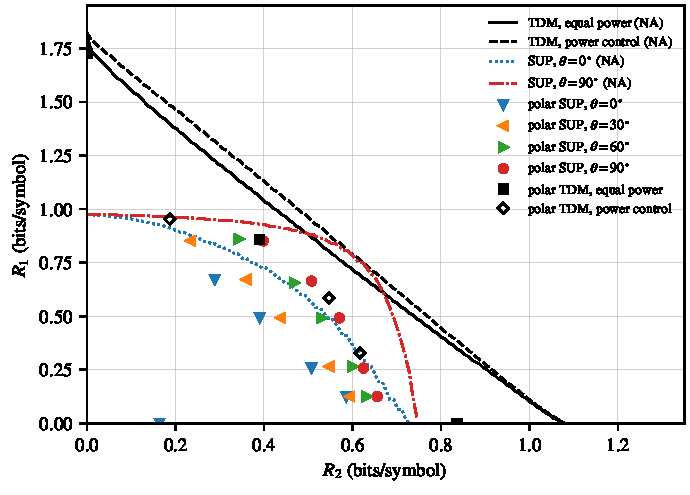
\includegraphics[width=0.78\textwidth]{figures/qam_realized_n128.pdf}
\caption{4-point AWGN broadcast channel at $7.33/2.15$~dB, $n=128$ symbols, $\varepsilon_1=\varepsilon_2=10^{-2}$: normal approximations (lines) and polar codes with SC decoding (markers).}
\label{fig:qam}
\end{figure}

\section{Discrete-domain superposition: the quaternary symmetric BC}\label{sec:qsbc}
\paragraph{Model.} $\mathrm{QSBC}(p_1,p_2)$: $Y_j=X+Z_j \pmod 4$ with $P(Z_j=0)=1-p_j$ and $P(Z_j=z)=p_j/3$ for $z\ne0$. The point-to-point capacity is $\Csf_{\QSC}(p)=2-h(p)-p\log_23$ and the dispersion $\Vsf_{\QSC}(p)=p(1-p)\log_2^2\frac{3(1-p)}{p}$. A $\QSC(p)$ is the composition of two $\QSC$s, so the channel is degraded. Matching the symbol error rate of hard-decided QPSK at the BSBC-matched SNRs gives $p_j=1-(1-q_j)^2$ with $q_j\in\{0.01,0.10\}$, i.e., $\mathrm{QSBC}(0.0199,0.19)$. Unlike Gray QPSK, the QSC corrupts both bits of a symbol together.

\paragraph{Superposition families.} The cloud $V$ is uniform on $\mathbb Z_4$ and $X=V+S\pmod 4$, with
\emph{symmetric} $S$: $P(S=0)=1-a$, $P(S=s)=a/3$;
\emph{subgroup} $S\in\{0,2\}$ with $P(S=2)=a$; and
\emph{bit-layer}: a binary cloud selects the pair $\{V,V+2\}$ and the satellite picks $V+2$ with probability $a$.
A random search over general $(P_V,P_{X|V})$ with $|\mathcal V|=4$ ($4\times10^5$ samples plus local refinement) checks whether the families reach the asymptotic boundary.

\paragraph{Results.} Table~\ref{tab:qsbc} gives the asymptotic advantage and the finite-$n$ advantage. The symmetric and subgroup families form the boundary, but general distributions exceed them by up to $0.026$ bits/symbol, so the true advantage is somewhat larger and the crossovers may come somewhat earlier than shown.

\begin{table}[t]
\centering
\caption{QSBC: largest $R_1$ advantage (bits/symbol) of SUP over TDM. The asymptotic value uses the structured families; ``RS'' is the further gain found by random search over general distributions. Finite-$n$ values are normal approximations with $\varepsilon_1=\varepsilon_2=10^{-2}$ over interior rate pairs; a negative value means SUP is dominated, and its size depends on how the interior is defined, so only the sign and the crossover are robust.}
\label{tab:qsbc}
\resizebox{\textwidth}{!}{%
\begin{tabular}{@{}lccrrrrrrr@{}}
\toprule
 & $n\to\infty$ & RS & $2^7$ & $2^8$ & $2^9$ & $2^{10}$ & $2^{11}$ & $2^{12}$ & $2^{13}$\\
\midrule
$\mathrm{QSBC}(0.0199,0.19)$ & $0.079$ & $+0.020$ & $-0.024$ & $-0.036$ & $-0.027$ & $-0.004$ & $+0.019$ & $+0.036$ & $+0.050$\\
$\mathrm{QSBC}(0.01,0.10)$ & $0.069$ & $+0.026$ & $-0.018$ & $-0.024$ & $-0.033$ & $-0.018$ & $-0.001$ & $+0.018$ & $+0.033$\\
$\mathrm{QSBC}(0.05,0.30)$ & $0.060$ & $+0.019$ & $<0$ & $<0$ & $<0$ & $+0.003$ & $+0.020$ & $+0.032$ & $+0.042$\\
\bottomrule
\end{tabular}}
\end{table}

\section{Binary versus quaternary at equal SNR}
Figure~\ref{fig:cross} compares the SUP advantage over TDM in QPSK symbols. In the binary model one QPSK symbol is two BSBC uses, so the BSBC curve is plotted at half its blocklength and twice its per-use rate. SUP first beats TDM at about $2^{10}$ symbols in the binary model and at $2^{11}$ in the quaternary model. Below the crossover the quaternary model's deficit is smaller under this metric (e.g., $-0.02$ against $-0.11$ bits/symbol at $2^7$ symbols), but that magnitude is metric-dependent; the crossover is not. The binary model's asymptotic advantage ($0.096$ bits/symbol) also exceeds the quaternary one ($0.079$, or up to about $0.10$ with optimized satellite distributions). The quaternary alphabet therefore does not shorten the blocklength at which superposition pays off.

\begin{figure}[t]
\centering
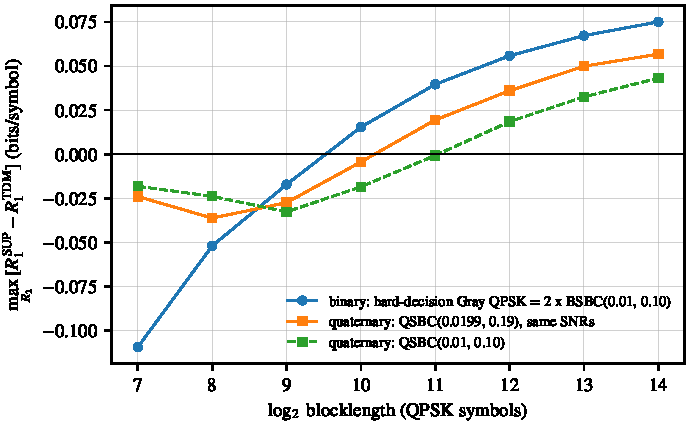
\includegraphics[width=0.78\textwidth]{figures/crossover_binary_vs_quaternary.pdf}
\caption{Largest $R_1$ advantage of SUP over TDM at equal $R_2$ (normal approximation, $\varepsilon_1=\varepsilon_2=10^{-2}$, interior rate pairs), in bits per QPSK symbol, against blocklength in QPSK symbols ($\ge2^7$). Interior pairs are those where both schemes have $R_1>0.02$.}
\label{fig:cross}
\end{figure}

\paragraph{Against CCP.} CCP is a weaker baseline, and SUP overtakes it much earlier (Table~\ref{tab:ccp}). In channel uses the quaternary model looks faster, but at equal SNR both cross at 32 QPSK symbols ($2^6$ BSBC uses versus $2^5$ QSBC symbols). These blocklengths are short enough that the normal approximation is only indicative. Entries marked $<0$ mean that SUP has no advantage at that blocklength.

\begin{table}[t]
\centering
\caption{Largest $R_1$ advantage of SUP over CCP (normal approximation, $\varepsilon=10^{-2}$), by blocklength in channel uses of each model.}
\label{tab:ccp}
\begin{tabular}{@{}lrrrrrr@{}}
\toprule
 & $2^5$ & $2^6$ & $2^7$ & $2^8$ & $2^9$ & $2^{10}$\\
\midrule
$\mathrm{BSBC}(0.01,0.10)$ (binary uses) & $<0$ & $+0.043$ & $+0.214$ & $+0.307$ & $+0.352$ & $+0.372$\\
$\mathrm{QSBC}(0.0199,0.19)$ (symbols) & $+0.349$ & $+0.387$ & $+0.625$ & $+0.733$ & $+0.787$ & $+0.809$\\
$\mathrm{QSBC}(0.01,0.10)$ (symbols) & $+0.234$ & $+0.231$ & $+0.402$ & $+0.487$ & $+0.524$ & $+0.534$\\
\bottomrule
\end{tabular}
\end{table}

\section{Discussion and implications for the paper}
\begin{itemize}
\item The paper's conclusion suggests that larger alphabets might make superposition more attractive. For 4-ary symbols this does not hold in either sense: the discrete construction needs the same or longer blocklength, and the power-domain construction's gains are power allocation that orthogonal access also obtains. The sentence should be revised, or replaced by the statement that at equal SNR a quaternary alphabet does not shorten the crossover.
\item The finding is consistent with Gaussian-channel results: Gorce \emph{et al.}~\cite{gorce2021noma} report that orthogonal access outperforms superposition at short blocklengths and below one bit per channel use; all channels here operate in or near that regime.
\item Uniform-bit power-domain superposition removes the satellite-selection problem of the Goela--Abbe--Gastpar construction, because each layer becomes an ordinary polar code. If the paper is reframed around when superposition pays off, this is worth a remark.
\item The natural next experiment is two bits per user per symbol (a hierarchical 16-QAM), where orthogonal I/Q splitting can no longer give each user a full dimension.
\end{itemize}

\section{Limitations}
\begin{itemize}
\item Normal approximations without third-order terms; values at $n\le64$ omitted. For the BSBC, adding $\frac12\log n/n$ to every constituent code did not move the TDM crossover.
\item The 4-point constellations are the parallelogram family $a(v)+b(s)$; other labelings of four points are not covered.
\item TDM with power control assumes an average power constraint across a user's slots.
\item The QSBC finite-$n$ curves use the structured families; general distributions add up to $0.026$ bits/symbol asymptotically.
\item Polar simulations: one SNR pair, $n=128$, SC decoding only, block error rates estimated from 6{,}000 blocks (about $\pm25\%$ relative at $10^{-2}$), rate resolution $1/128$.
\item The quaternary channel is the fully symmetric QSC. Other 4-ary channels (e.g., with adjacent-symbol errors more likely than diagonal ones) may behave differently.
\end{itemize}

\section{Reproducibility}
All scripts are in \texttt{scripts/} of the repository and need only numpy and matplotlib.
\begin{itemize}
\item \texttt{qam\_bc.py}, \texttt{qam\_sweep.py}: 4-point AWGN normal approximations; results in \texttt{qam\_sweep\_results.txt}.
\item \texttt{qam\_polar\_sim.py}, \texttt{qam\_realized.py}: polar encoder, SC decoder, genie construction and rate search; \texttt{python3 qam\_realized.py 7.33 2.15 128} gives \texttt{qam\_realized\_7.33dB\_2.15dB\_n128.txt} (about 10 minutes).
\item \texttt{qsbc.py}, \texttt{qsbc\_sweep.py}: QSBC moments, families, random search and normal approximations; results in \texttt{qsbc\_sweep\_results.txt}.
\item \texttt{sup\_vs\_ccp.py}: Table~\ref{tab:ccp}. \texttt{interior\_gaps.py}: the curves of Figure~\ref{fig:cross} and the finite-$n$ entries of Table~\ref{tab:qsbc}.
\item \texttt{make\_report\_figures.py}: both figures.
\end{itemize}

\bibliographystyle{IEEEtran}
\bibliography{../refs}
\end{document}
